\section{Definitions and Notations}


\textbf{Planar Graph:} A graph $G = (V, E)$ is defined as \textit{planar} if it can be drawn on the Euclidean plane $\mathbb{R}^2$ without any edges crossing except at their endpoints (vertices). The term describes a topological property of the graph itself rather than a particular drawing of it. In other words, a graph is called planar if there exists at least one way to represent it in the plane so that no two edges intersect improperly.

It is crucial to distinguish the graph's inherent planarity from its visual representation; a planar graph may be rendered with edge crossings in a given drawing, yet it remains planar as long as at least one crossing-free configuration exists. Conversely, \textit{non-planar graphs} cannot be drawn without at least one intersection, regardless of the arrangement. The most fundamental examples of non-planar graphs are the complete graph $K_5$ and the complete bipartite graph $K_{3,3}$ shown in Figure~\ref{fig:nonplanar}.

\begin{figure}
\centering
% ----------- K5 -----------
\begin{subfigure}[t]{0.45\linewidth}
\centering
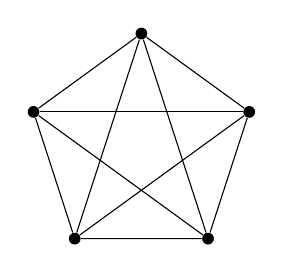
\begin{tikzpicture}[scale=1.2, every node/.style={circle, fill=black, inner sep=1.5pt}]
    \foreach \i in {1,...,5}
        \node (v\i) at ({90-(\i-1)*72}:1.2) {};
    
    \draw (v1)--(v2)--(v3)--(v4)--(v5)--(v1);
    \draw (v1)--(v3);
    \draw (v1)--(v4);
    \draw (v2)--(v4);
    \draw (v2)--(v5);
    \draw (v3)--(v5);
\end{tikzpicture}
\caption{The complete graph $K_5$}
\end{subfigure}
\hfill
% ----------- K3,3 -----------
\begin{subfigure}[t]{0.45\linewidth}
\centering
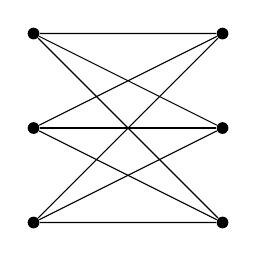
\begin{tikzpicture}[scale=1.2, every node/.style={circle, fill=black, inner sep=1.5pt}]
    \foreach \i in {1,2,3} {
        \node (a\i) at (0, \i-2) {};
        \node (b\i) at (2, \i-2) {};
    }
    \foreach \i in {1,2,3}
        \foreach \j in {1,2,3}
            \draw (a\i)--(b\j);
\end{tikzpicture}
\caption{The bipartite graph $K_{3,3}$}
\end{subfigure}
\caption{The two minimal non-planar graphs shown with unavoidable edge crossings.}
\label{fig:nonplanar}
\end{figure}

\textbf{Plane Graph:} While "planar" refers to the capacity of the graph to be drawn without crossings, a \textit{plane graph} refers to a specific \textit{planar embedding} (or drawing) of that graph in which no two edges intersect except at their endpoints. 

As illustrated by the complete graph $K_4$ in Figure~\ref{fig:k4_example}, a single planar graph can yield multiple representations. A drawing of $K_4$ in a standard rectilinear format typically results in an edge crossing; however, by relocating a single vertex or routing an edge externally, a crossing-free "plane" representation is achieved. This demonstrates that while $K_4$ is fundamentally a planar graph, only specific drawings of it constitute plane graphs.

\begin{figure}
\centering
% ----------- Planar embedding of K4 -----------
\begin{subfigure}[t]{0.45\linewidth}
\centering
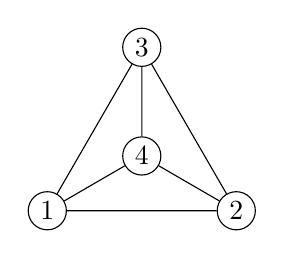
\begin{tikzpicture}[scale=1.2, every node/.style={circle, draw, fill=white, inner sep=2pt}]
    \node (v1) at (0,0) {1};
    \node (v2) at (2,0) {2};
    \node (v3) at (1,1.73) {3};
    \node (v4) at (1,0.58) {4};
    
    \draw (v1)--(v2)--(v3)--(v1);
    \draw (v1)--(v4);
    \draw (v2)--(v4);
    \draw (v3)--(v4);
\end{tikzpicture}
\caption{A plane embedding of $K_4$}
\label{fig:k4_planar}
\end{subfigure}
\hfill
% ----------- Non-planar drawing of K4 -----------
\begin{subfigure}[t]{0.45\linewidth}
\centering
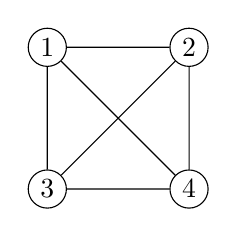
\begin{tikzpicture}[scale=1.2, every node/.style={circle, draw, fill=white, inner sep=2pt}]
    \node (v1) at (0,1.5) {1};
    \node (v2) at (1.5,1.5) {2};
    \node (v3) at (0,0) {3};
    \node (v4) at (1.5,0) {4};
    
    \draw (v1)--(v2)--(v4)--(v3)--(v1);
    \draw (v1)--(v4);
    \draw (v2)--(v3);
\end{tikzpicture}
\caption{A non-plane drawing of $K_4$}
\label{fig:k4_nonplanar}
\end{subfigure}
\caption{Verification of the planarity of $K_4$: (a) provides a valid plane embedding, while (b) illustrates a drawing with a crossing that does not alter the graph's underlying planarity.}
\label{fig:k4_example}
\end{figure}


A plane graph divides the plane into distinct areas called \emph{regions} (also known as \emph{faces}, \emph{windows}, or \emph{meshes}). Each region is defined by the set of edges forming its boundary. For example, the graph shown in Figure~\ref{fig:plane_graph} contains three such regions:

\begin{align*}
R_1 = (&(v_1, v_2), (v_2, v_4), (v_4, v_5), (v_5, v_6), (v_6, v_1)) \\
R_2 = (&(v_1, v_6), (v_6, v_3), (v_3, v_1)) \\
R_3 = (&(v_1, v_3), (v_3, v_6), (v_6, v_5), (v_5, v_4), (v_4, v_2), \\
&(v_2, v_1))
\end{align*}


\begin{figure}
    \centering
    \begin{tikzpicture}
        % vertices
        \coordinate (v1) at (0,4.5);
        \coordinate (v2) at (-1.5,2.5);
        \coordinate (v3) at (3,3);
        \coordinate (v4) at (-1,1);
        \coordinate (v5) at (1,0);
        \coordinate (v6) at (2.5, 0.5);
        
        % edges
        \draw (v1) -- (v2);
        \draw (v1) -- (v6);
        \draw (v3) -- (v1);
        \draw (v2) -- (v4);
        \draw (v4) -- (v5);
        \draw (v5) -- (v6);
        \draw (v6) -- (v3);
        
        % labels with math mode
        \foreach \v/\pos/\labeltext in {v1/above/$v_1$, v2/left/$v_2$, v3/right/$v_3$, v4/below left/$v_4$, v5/below/$v_5$, v6/below right/$v_6$}
        {    
            \node[\pos] at (\v) {\labeltext};
            \fill (\v) circle[radius=2pt];  % black filled circle
        }
        
        % regions - lightly shaded for clarity
        \begin{scope}
            \filldraw[fill=gray!60,opacity=0.3] (v1) -- (v2) -- (v4) -- (v5) -- (v6) -- cycle;
            \filldraw[fill=gray!30,opacity=0.3] (v1) -- (v6) -- (v3) -- cycle;
            % The exterior region outside edges can be left unshaded
        \end{scope}
            
        % edge labels (midpoints)
        \node[left] at ($(v1)!0.5!(v2)$) {$e_1$};
        \node[right] at ($(v1)!0.5!(v3)$) {$e_2$};
        \node[left] at ($(v1)!0.5!(v6)$) {$e_3$};
        \node[left] at ($(v2)!0.5!(v4)$) {$e_4$};
        \node[right] at ($(v3)!0.5!(v6)$) {$e_5$};
        \node[below] at ($(v5)!0.5!(v4)$) {$e_6$};
        \node[below] at ($(v5)!0.5!(v6)$) {$e_7$};
        
        % region labels (inside faces)
        \node at (0,2) {$R_1$}; % triangle top region
        \node at (2,2.5) {$R_2$};   % quadrilateral below
        \node at (3.5,3.75) {$R_3$}; % exterior region (optional)
        
    \end{tikzpicture}
    \caption{Plane graph with seven edges forming three regions.}
    \label{fig:plane_graph}
\end{figure}

Among them, \( R_3 \) is called the \emph{exterior region}, which lies outside the boundary of the graph.
Given two edges \( e_1 = (v_i, v_j) \) and \( e_2 = (v_j, v_k) \); if rotating \( e_1 \) in a clockwise direction around the shared vertex \( v_j \) toward \( e_2 \) does not encounter any other edge incident on \( v_j \), then the area enclosed between \( e_1 \) and \( e_2 \) defines a \emph{wedge}, denoted \( (v_i, v_j, v_k) \). Two wedges such as \( (v_i, v_j, v_k) \) and \( (v_j, v_k, v_l) \) are called contiguous.
In any plane graph with \( m \) edges, there are exactly \( 2m \) wedges. Returning to the graph in Figure~\ref{fig:plane_graph}, which has 7 edges, we find 14 wedges:
\begin{align*}
& (v_2, v_1, v_3),\ (v_3, v_1, v_6),\ (v_6, v_1, v_2),\ (v_4, v_2, v_1), \\
&  (v_1, v_2, v_4),\ (v_1, v_3, v_6),\ (v_6, v_3, v_1),\ (v_2, v_4, v_5), \\
& (v_5, v_4, v_2),\ (v_4, v_5, v_6),\ (v_6, v_5, v_4),\ (v_1, v_6, v_3), \\
& (v_3, v_6, v_5),\ (v_5, v_6, v_1)
\end{align*}
Each region in a plane graph can be represented in any one of the three equivalent ways:
\begin{itemize}
    \item As a sequence of \emph{vertices}
    \item As a sequence of \emph{edges}
    \item Or as a sequence of \emph{wedges}.
\end{itemize}
For example, region \( R_1 \) from Figure~\ref{fig:plane_graph} can be expressed as:
\begin{align*}
(&v_1, v_2, v_4, v_5, v_6), \\
(&(v_1, v_2), (v_2, v_4), (v_4, v_5), (v_5, v_6), (v_6, v_1)), \text{ or } \\
(&(v_1, v_2, v_4), (v_2, v_4, v_5), (v_4, v_5, v_6), (v_5, v_6, v_1),\\
&(v_6, v_1, v_2))
\end{align*}
The three representations are equivalent and can be easily transformed into each other. Thus, either of them can be chosen for convenience.

\textbf{Half-Edge:} In the context of computational geometry, a half-edge is a directed representation of an edge. It is like a general directed edge, but additionally, it points to the next half-edge, which allows a "walk" around any polygon.

\textbf{Twin Edge:} Every half-edge $e = \langle u, v \rangle$ that originates at the vertex $u$ and ends at the vertex $v$ is associated with a unique \textit{twin edge} $\bar{e} = \langle v, u \rangle$. The twin edge originates at $v$ and ends at $u$, representing the same geometric span but oriented in the opposite direction. Figure~\ref{fig:half_edges} illustrates half-edges and their twin edges of a triangle.

\begin{figure}
    \centering
    \begin{tikzpicture}[
        vertex/.style={circle, fill=black, inner sep=1.5pt},
        thisedge/.style={->, >=Stealth, shorten >=4pt, thick, shorten <=4pt},
        halfedge/.style={->, >=Stealth, shorten >=4pt, shorten <=4pt},
        twinedge/.style={->, >=Stealth, shorten >=4pt, dashed, shorten <=4pt},
        % nextarrow/.style={->, >=latex, dashed, orange}
        nextarrow/.style={->, orange},
        edgeLabel/.style={midway, sloped, font=\scriptsize, inner sep=2pt}
    ]
        % Vertices
        \node[vertex, label=left:$v_i$] (vi) at (0,0) {};
        \node[vertex, label=right:$v_j$] (vj) at (4,0) {};
        \node[vertex, label=above:$v_k$] (vk) at (2, 2) {};

        % Half-edges (twins)
        \draw[thisedge, transform canvas={yshift=-3pt}] (vi) -- (vj) node[edgeLabel, below] {this};
        \draw[twinedge, transform canvas={yshift=3pt}] (vj) -- (vi) node[edgeLabel, above] {this.twin};

        \draw[halfedge, transform canvas={xshift=3pt}] (vj) -- (vk) node[edgeLabel, above] {this.next};
        \draw[twinedge, transform canvas={xshift=-3pt}] (vk) -- (vj) node[edgeLabel, below] {this.next.twin};

        \draw[halfedge, transform canvas={xshift=-3pt}] (vk) -- (vi) node[edgeLabel, above] {this.next.next};
        \draw[twinedge, transform canvas={xshift=3pt}] (vi) -- (vk) node[edgeLabel, below] {this.twin.next};        
    \end{tikzpicture}
    \caption{An illustration of half-edges and their twin edges of a triangle}
    \label{fig:half_edges}
\end{figure}